\chapter{Results}
\label{chapter:6}

After the implementation described in the last chapter, it was possible
to achieve initial federation functionality that showcases the
possibilities of federation using the Diaspora protocol. This proof of
concept counts with the following features.

\textit{Remote users can be found using Noosfero search} using the user
identifier and the remote pod host name (Figure
\ref{fig:noosfero_search}). Remote profiles are created to store and
display the public info in the local server.

\begin{figure}[hbt]
  \centering
  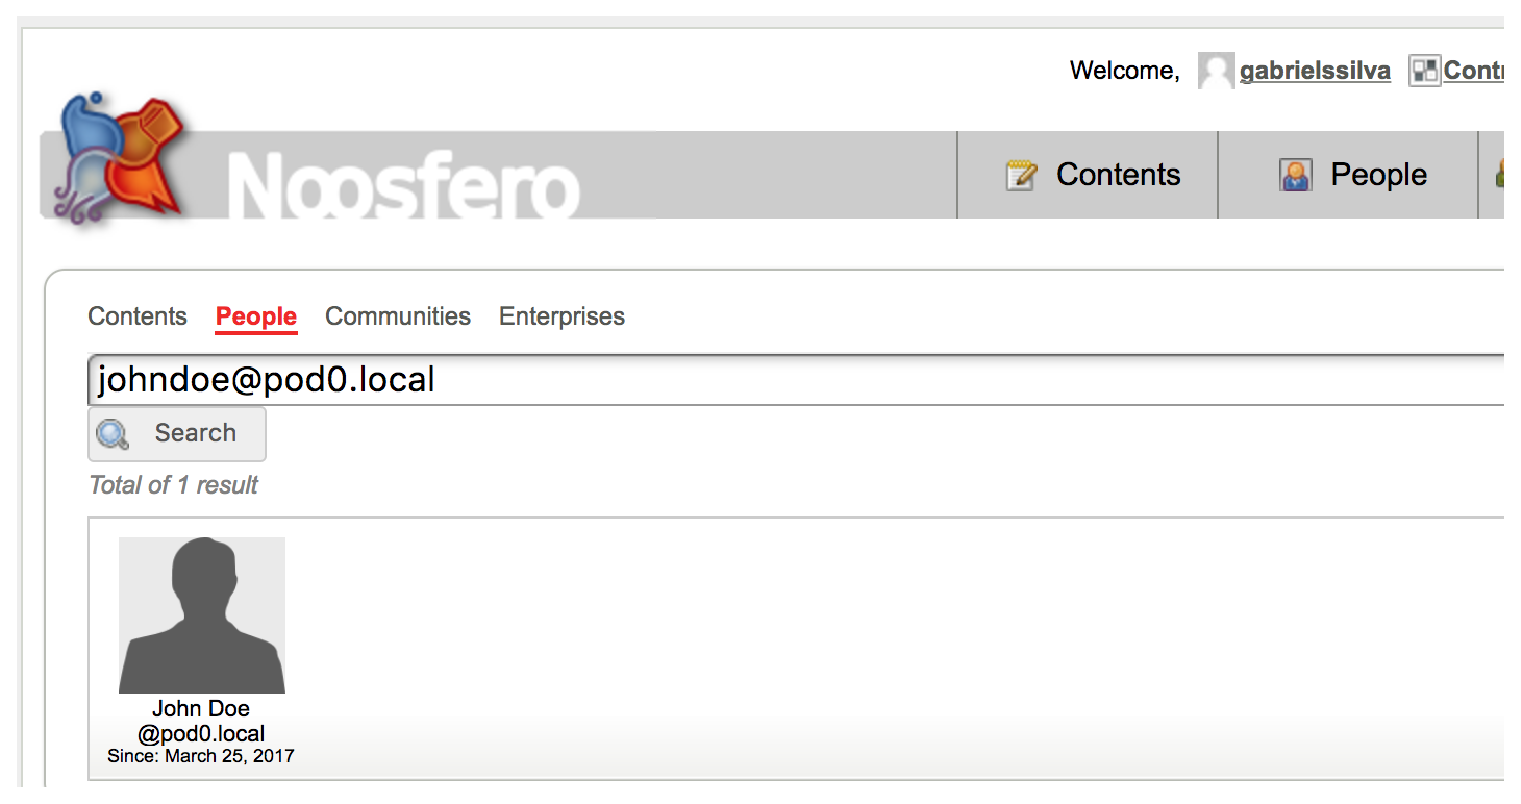
\includegraphics[width=0.5\textwidth]{figures/noosfero_search.eps}
  \caption{Diaspora user displayed in Noosfero search results}
  \label{fig:noosfero_search}
\end{figure}

\textit{Noosfero users can also be found on the Diaspora side}, since Noosfero
servers now respond to WebFinger and hCard requests (Figure
\ref{fig:diaspora_search}).

\begin{figure}[hbt]
  \centering
    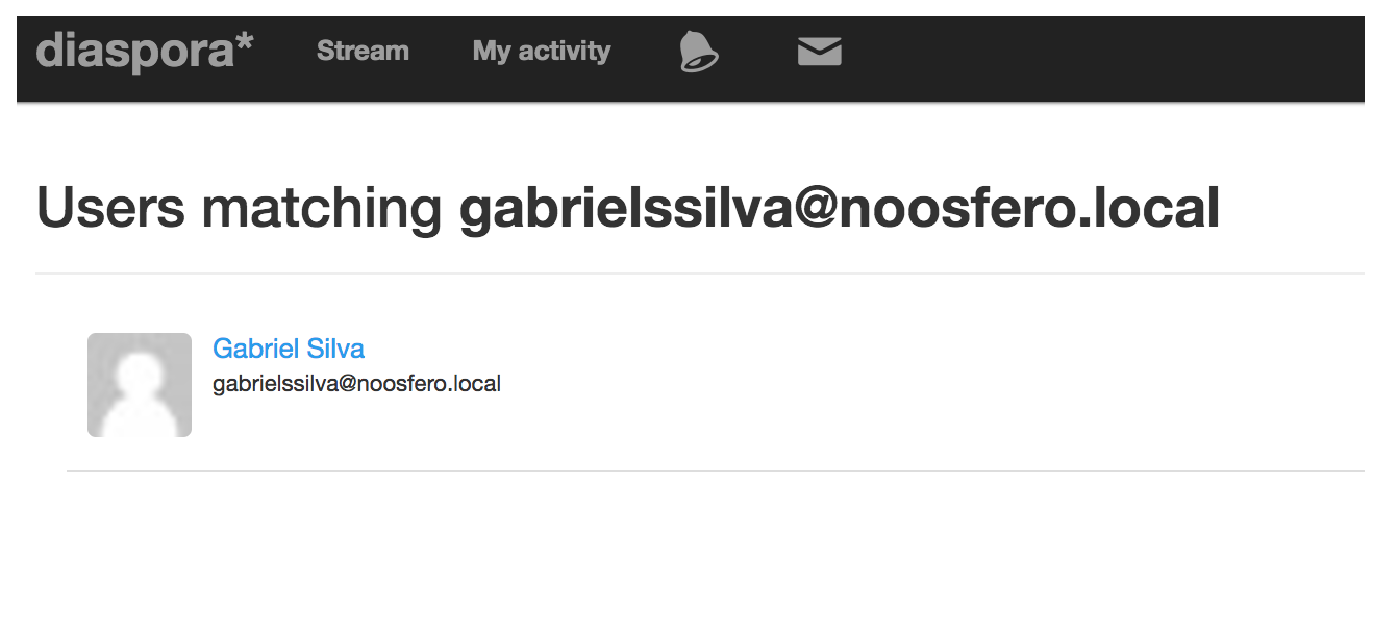
\includegraphics[width=0.5\textwidth]{figures/diaspora_search.eps}
  \caption{Noosfero users displayed in Diaspora search results}
  \label{fig:diaspora_search}
\end{figure}

\textit{Remote users can be followed by users of a Noosfero server}. When
following a remote user, Noosfero notifies the remote server, which will
handle the message by creating the relationship and notifying the
related users. Figure \ref{fig:diaspora_notification} shows a
notification displayed for a Diaspora user after he was discovered and
followed by a remote Noosfero server.

\begin{figure}[hbt]
  \centering
    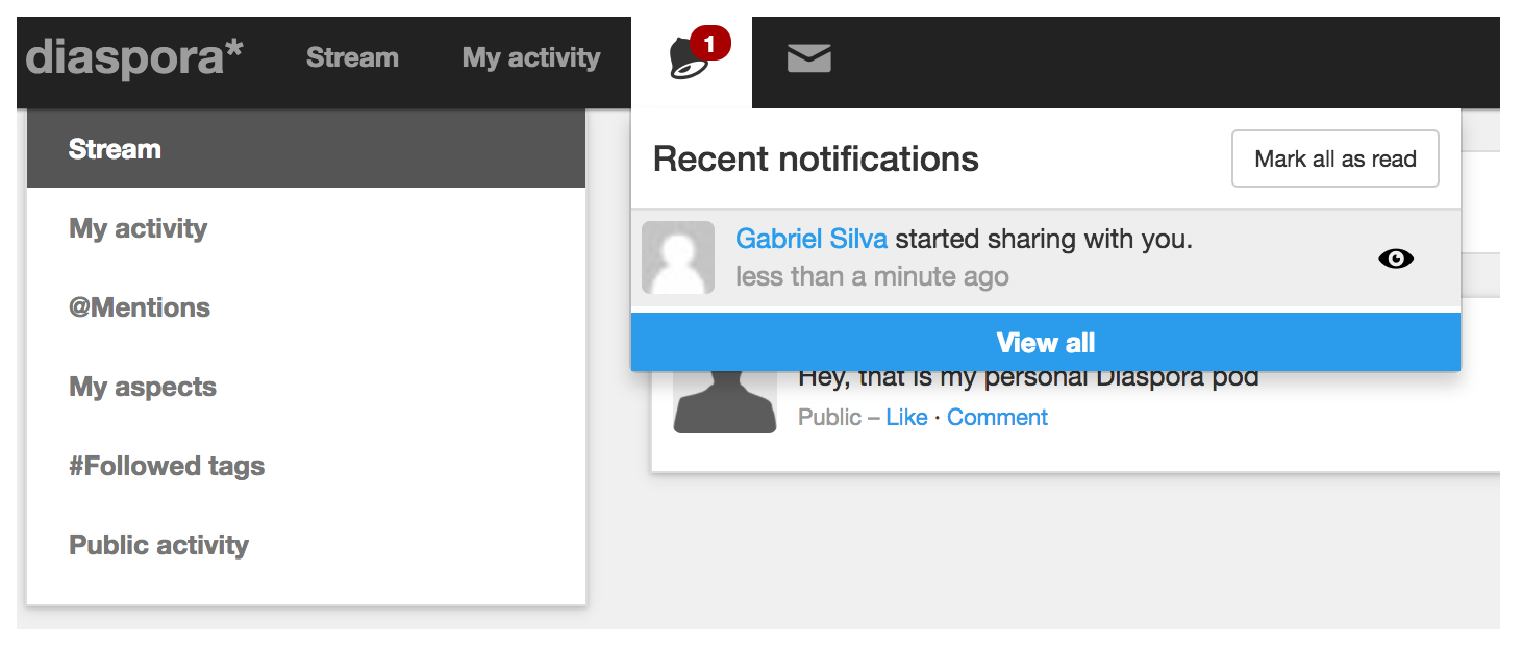
\includegraphics[width=0.5\textwidth]{figures/diaspora_notification.eps}
  \caption{Notification of remote activity in Diaspora}
  \label{fig:diaspora_notification}
\end{figure}

\textit{Any content created by Diaspora users being followed by someone in the
local server will be sent to Noosfero}, that will handle them by creating
the content locally. The publication is displayed in the remote user
local profile, but notifications can also be sent to all related users
(Figure \ref{fig:noosfero_remote_wall}).

As users are able to reply existing publications, comments must also be sent
to remote servers. \textit{Noosfero will create comments locally, and send
comments to other servers} when remote users are subscribed. Publications
and comments are both important for a first set of federation features.

\begin{figure}[hbt]
  \centering
    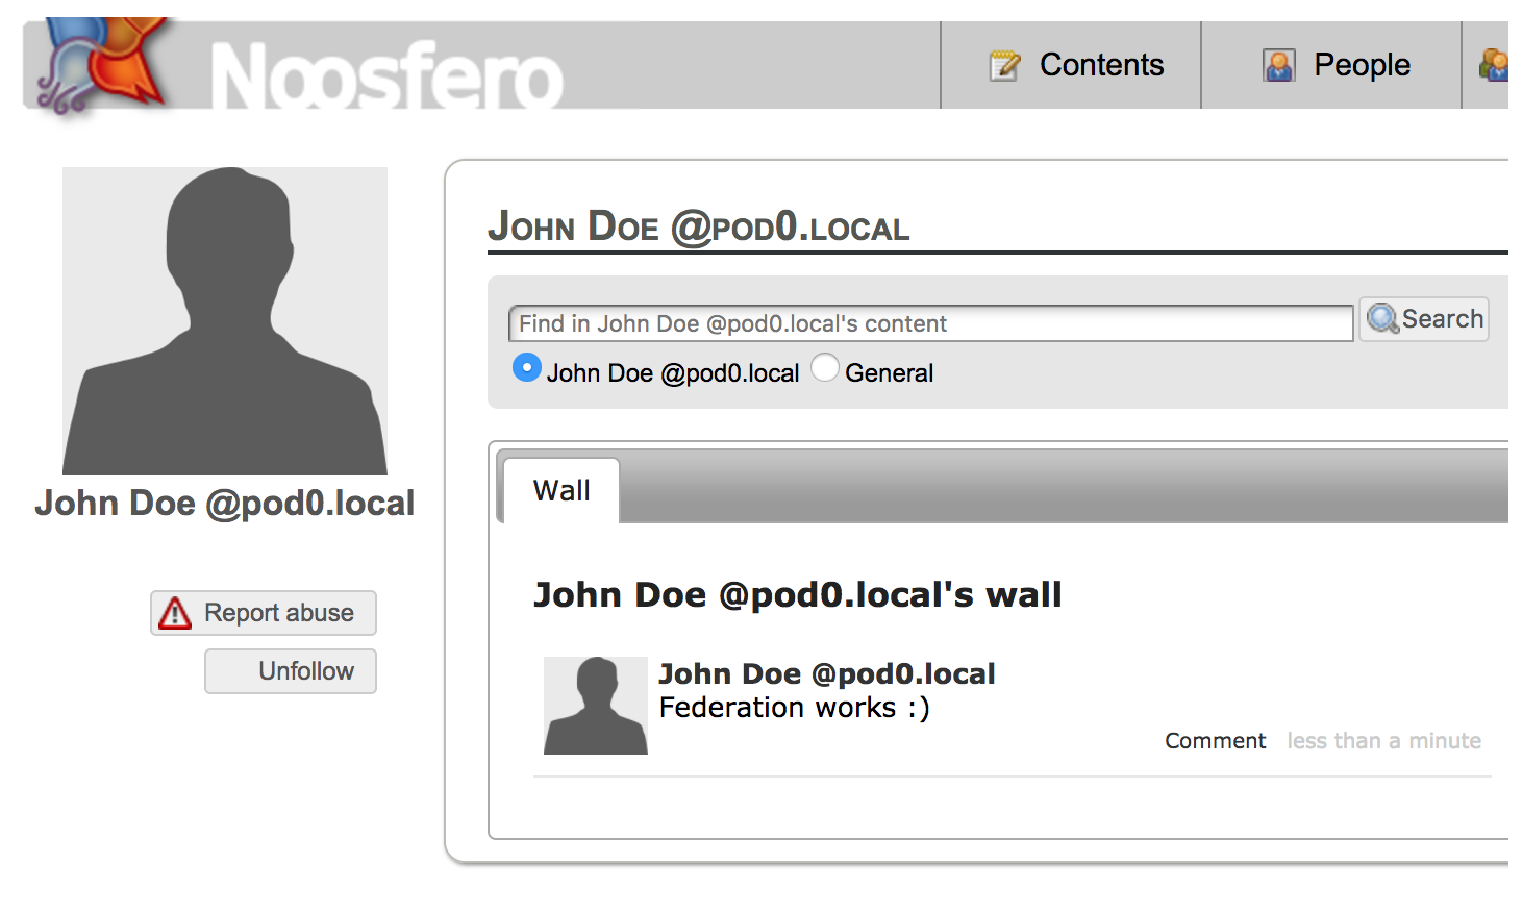
\includegraphics[width=0.5\textwidth]{figures/noosfero_remote_wall.eps}
  \caption{Content created by Diaspora users displayed in Noosfero}
  \label{fig:noosfero_remote_wall}
\end{figure}

The information sent by other servers is usually saved to the local database, so
there will be an amount of data replication, requiring further attention to maintain
coherence across the network. Users can delete publications or comments, edit their
personal information, unfollow other users and even destroy their own account. These
tractions are also represented as entities that are handled by Noosfero, which also
sends them accordingly.

These features will work between Noosfero and any application that
supports the Diaspora protocol, not only Diaspora itself. User discovery
will work with any server that supports the WebFinger and hCard
standards as well.
